
\documentclass[]{article}
\voffset=-1.5cm
\oddsidemargin=0.0cm
\textwidth = 480pt

% http://www.strath.ac.uk/aer/materials/5furtherquantitativeresearchdesignandanalysis/unit6/whatislogisticregression/

% http://www.medcalc.org/manual/logistic_regression.php


\usepackage{amsmath}
\usepackage{graphicx}
\usepackage{amssymb}
\usepackage{framed}
\usepackage{multicol}
%\usepackage[paperwidth=21cm, paperheight=29.8cm]{geometry}
%\usepackage[angle=0,scale=1,color=black,hshift=-0.4cm,vshift=15cm]{background}
%\usepackage{multirow}
\usepackage{enumerate}






\begin{document}
Introduction
The Pearson product-moment correlation coefficient (Pearson’s correlation, for short) is a measure of the strength and direction of association that exists between two variables measured on at least an interval scale.

For example, you could use a Pearson’s correlation to understand whether there is an association between exam performance and time spent revising. You could also use a Pearson's correlation to understand whether there is an association between depression and length of unemployment.

A Pearson’s correlation attempts to draw a line of best fit through the data of two variables, and the Pearson correlation coefficient, r, indicates how far away all these data points are from this line of best fit (i.e., how well the data points fit this model/line of best fit). You can learn more here, which we recommend if you are not familiar with this test.

Note: If one of your two variables is dichotomous you can use a point-biserial correlation instead, or if you have one or more control variables, you can run a Pearson's partial correlation.

This "quick start" guide shows you how to carry out a Pearson's correlation using SPSS Statistics, as well as interpret and report the results from this test. However, before we introduce you to this procedure, you need to understand the different assumptions that your data must meet in order for a Pearson's correlation to give you a valid result. We discuss these assumptions next.

\section{Pearson Product-Moment Correlation}

What does this test do?
The Pearson product-moment correlation coefficient (or Pearson correlation coefficient, for short) is a measure of the strength of a linear association between two variables and is denoted by r. Basically, a Pearson product-moment correlation attempts to draw a line of best fit through the data of two variables, and the Pearson correlation coefficient, r, indicates how far away all these data points are to this line of best fit (i.e., how well the data points fit this new model/line of best fit).

What values can the Pearson correlation coefficient take?
The Pearson correlation coefficient, r, can take a range of values from +1 to -1. A value of 0 indicates that there is no association between the two variables. A value greater than 0 indicates a positive association; that is, as the value of one variable increases, so does the value of the other variable. A value less than 0 indicates a negative association; that is, as the value of one variable increases, the value of the other variable decreases. This is shown in the diagram below:

Pearson Coefficient - Different Values 

How can we determine the strength of association based on the Pearson correlation coefficient?
The stronger the association of the two variables, the closer the Pearson correlation coefficient, r, will be to either +1 or -1 depending on whether the relationship is positive or negative, respectively. Achieving a value of +1 or -1 means that all your data points are included on the line of best fit – there are no data points that show any variation away from this line. Values for r between +1 and -1 (for example, r = 0.8 or -0.4) indicate that there is variation around the line of best fit. The closer the value of r to 0 the greater the variation around the line of best fit. Different relationships and their correlation coefficients are shown in the diagram below:

Different values for the Pearson Correlation Coefficient 

%====================================================%

Are there guidelines to interpreting Pearson's correlation coefficient?
Yes, the following guidelines have been proposed:

 	Coefficient, r
Strength of 	Positive	Negative
Association
Small	.1 to .3	-0.1 to -0.3
Medium	.3 to .5	-0.3 to -0.5
Large	.5 to 1.0	-0.5 to -1.0

Remember that these values are guidelines and whether an association is strong or not will also depend on what you are measuring.

Can you use any type of variable for Pearson's correlation coefficient?
No, the two variables have to be measured on either an interval or ratio scale. However, both variables do not need to be measured on the same scale (e.g., one variable can be ratio and one can be interval). Further information about types of variable can be found in our Types of Variable guide. If you have ordinal data, you will want to use Spearman's rank-order correlation or a Kendall's Tau Correlation instead of the Pearson product-moment correlation.

Do the two variables have to be measured in the same units?
No, the two variables can be measured in entirely different units. For example, you could correlate a person's age with their blood sugar levels. Here, the units are completely different; age is measured in years and blood sugar level measured in mmol/L (a measure of concentration). Indeed, the calculations for Pearson's correlation coefficient were designed such that the units of measurement do not affect the calculation. This allows the correlation coefficient to be comparable and not influenced by the units of the variables used.

What about dependent and independent variables?
The Pearson product-moment correlation does not take into consideration whether a variable has been classified as a dependent or independent variable. It treats all variables equally. For example, you might want to find out whether basketball performance is correlated to a person's height. You might, therefore, plot a graph of performance against height and calculate the Pearson correlation coefficient. Lets say, for example, that r = .67. That is, as height increases so does basketball performance. This makes sense. However, if we plotted the variables the other way around and wanted to determine whether a person's height was determined by their basketball performance (which makes no sense), we would still get r = .67. This is because the Pearson correlation coefficient makes no account of any theory behind why you chose the two variables to compare. This is illustrated below:

Not influenced by Dependent and Independent Variables 

Does the Pearson correlation coefficient indicate the slope of the line?
It is important to realize that the Pearson correlation coefficient, r, does not represent the slope of the line of best fit. Therefore, if you get a Pearson correlation coefficient of +1 this does not mean that for every unit increase in one variable there is a unit increase in another. It simply means that there is no variation between the data points and the line of best fit. This is illustrated below:

The Pearson Coefficient does not indicate the slope of the line of best fit. 

%============================================================%
\subsection{Assumptions}


What assumptions does Pearson's correlation make?
There are five assumptions that are made with respect to Pearson's correlation:

The variables must be either interval or ratio measurements (see our Types of Variable guide for further details).
The variables must be approximately normally distributed (see our Testing for Normality guide for further details).
There is a linear relationship between the two variables (but see note at bottom of page). We discuss this later in this guide (jump to this section here).
Outliers are either kept to a minimum or are removed entirely. We also discuss this later in this guide (jump to this section here).
There is homoscedasticity of the data. This is discussed later in this guide (jump to this section here).
How can you detect a linear relationship?
To test to see whether your two variables form a linear relationship you simply need to plot them on a graph (a scatterplot, for example) and visually inspect the graph's shape. In the diagram below, you will find a few different examples of a linear relationship and some non-linear relationships. It is not appropriate to analyse a non-linear relationship using a Pearson product-moment correlation.

Detecting a Linear Relationship. 

Note: Pearson's correlation determines the degree to which a relationship is linear. Put another way, it determines whether there is a linear component of association between two continuous variables. As such, linearity is not actually an assumption of Pearson's correlation. However, you would not normally want to pursue a Pearson's correlation to determine the strength and direction of a linear relationship when you already know the relationship between your two variables is not linear. Instead, the relationship between your two variables might be better described by another statistical measure. For this reason, it is not uncommon to view the relationship between your two variables in a scatterplot to see if running a Pearson's correlation is the best choice as a measure of association or whether another measure would be better.

%==============================================================%
Pearson Product-Moment Correlation (cont...)

How can you detect outliers?
An outlier (in correlation analysis) is a data point that does not fit the general trend of your data, but would appear to be a wayward (extreme) value and not what you would expect compared to the rest of your data points. You can detect outliers in a similar way to how you detect a linear relationship, by simply plotting the two variables against each other on a graph and visually inspecting the graph for wayward (extreme) points. You can then either remove or manipulate that particular point as long as you can justify why you did so (there are far more robust methods for detecting outliers in regression analysis). Alternatively, if you cannot justify removing the data point(s), you can run a nonparametric test such as Spearman's rank-order correlation or Kendall's Tau Correlation instead, which are much less sensitive to outliers. This might be your best approach if you cannot justify removing the outlier. The diagram below indicates what a potential outlier might look like:

An outlier in Correlation. 

Why is testing for outliers so important?
Outliers can have a very large effect on the line of best fit and the Pearson correlation coefficient, which can lead to very different conclusions regarding your data. This point is most easily illustrated by studying scatterplots of a linear relationship with an outlier included and after its removal, with respect to both the line of best fit and the correlation coefficient. This is illustrated in the diagram below:

The effect of an outlier in Correlation. 

%==================================================================%


\subsection{What is homoscedasticity?}
Homoscedasticity basically means that the variances along the line of best fit remain similar as you move along the line. It is required that your data show homoscedasticity for you to run a Pearson product-moment correlation. Homoscedasticity is most easily demonstrated diagrammatically as below:

\subsection{Homoscedasticity in Correlation.} 

Can you establish cause-and-effect?
No, the Pearson correlation cannot determine a cause-and-effect relationship. It can only establish the strength of linear association between two variables. As stated earlier, it does not even distinguish between independent and dependent variables.

How do I report the output of a Pearson product-moment correlation?
You need to state that you used the Pearson product-moment correlation and report the value of the correlation coefficient, r, as well as the degrees of freedom (df). You should express the result as follows:

Expressing the Pearson Correlation. 

where the degrees of freedom (df) is the number of data points minus 2 (N – 2). If you have not tested the significance of the correlation then leave out the degrees of freedom and p-value such that you would simply report: r = -0.52.

%================================================================%


Can I determine whether the association is statistically significant?
Yes, the easy way to do this is through a statistical programme, such as SPSS Statistics. We provide a guide on how to do this, which you can find here. You need to be careful how you interpret the statistical significance of a correlation. If your correlation coefficient has been determined to be statistically significant this does not mean that you have a strong association. It simply tests the null hypothesis that there is no relationship. By rejecting the null hypothesis, you accept the alternative hypothesis that states that there is a relationship, but with no information about the strength of the relationship or its importance.

What is the Coefficient of Determination?
The coefficient of determination, r2, is the square of the Pearson correlation coefficient r (i.e., r2). So, for example, a Pearson correlation coefficient of 0.6 would result in a coefficient of determination of 0.36, (i.e., r2 = 0.6 x 0.6 = 0.36). The coefficient of determination, with respect to correlation, is the proportion of the variance that is shared by both variables. It gives a measure of the amount of variation that can be explained by the model (the correlation is the model). It is sometimes expressed as a percentage (e.g., 36\% instead of 0.36) when we discuss the proportion of variance explained by the correlation. However, you should not write r2 = 36%, or any other percentage. You should write it as a proportion (e.g., r2 = 0.36).

To run a Pearson correlation in SPSS Statistics, go to our guide here.

%====================================================================%


\subsection{Assumptions}
When you choose to analyse your data using Pearson’s correlation, part of the process involves checking to make sure that the data you want to analyse can actually be analysed using Pearson’s correlation. You need to do this because it is only appropriate to use Pearson’s correlation if your data "passes" four assumptions that are required for Pearson’s correlation to give you a valid result. In practice, checking for these four assumptions just adds a little bit more time to your analysis, requiring you to click of few more buttons in SPSS Statistics when performing your analysis, as well as think a little bit more about your data, but it is not a difficult task.

Before we introduce you to these four assumptions, do not be surprised if, when analysing your own data using SPSS Statistics, one or more of these assumptions is violated (i.e., is not met). 

This is not uncommon when working with real-world data rather than textbook examples, which often only show you how to carry out Pearson’s correlation when everything goes well! However, don’t worry. Even when your data fails certain assumptions, there is often a solution to overcome this. First, let’s take a look at these four assumptions:

\begin{description}
	\item[Assumption 1:]  Your two variables should be measured at the interval or ratio level (i.e., they are continuous). Examples of variables that meet this criterion include revision time (measured in hours), intelligence (measured using IQ score), exam performance (measured from 0 to 100), weight (measured in kg), and so forth. You can learn more about interval and ratio variables in our Types of Variable guide.
	
	\item[Assumption 2:] There is a linear relationship between your two variables. Whilst there are a number of ways to check whether a linear relationship exists between your two variables, we suggest creating a scatterplot using SPSS Statistics, where you can plot the one variable against the other variable, and then visually inspect the scatterplot to check for linearity. Your scatterplot may look something like one of the followingdescription
\end{description}
:
\begin{figure}
\centering
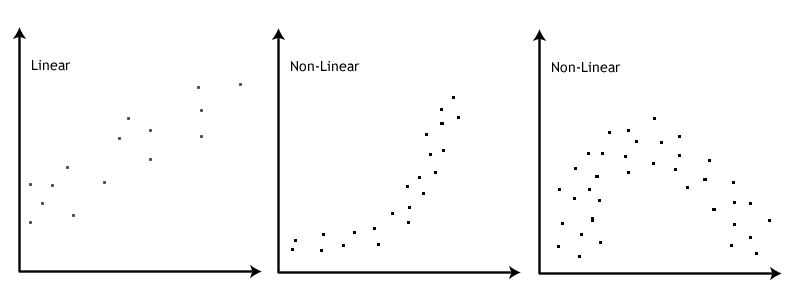
\includegraphics[width=0.7\linewidth]{images/linear-non-linear}
\end{figure}

If the relationship displayed in your scatterplot is not linear, you will have to either run a nonparametric equivalent to Pearson’s correlation or transform your data, which you can do using SPSS Statistics. In our enhanced guides, we show you how to: (a) create a scatterplot to check for linearity when carrying out Pearson’s correlation using SPSS Statistics; (b) interpret different scatterplot results; and (c) transform your data using SPSS Statistics if there is not a linear relationship between your two variables.

Note: Pearson's correlation determines the degree to which a relationship is linear. Put another way, it determines whether there is a linear component of association between two continuous variables. As such, linearity is not actually an assumption of Pearson's correlation. 

However, you would not normally want to pursue a Pearson's correlation to determine the strength and direction of a linear relationship when you already know the relationship between your two variables is not linear. Instead, the relationship between your two variables might be better described by another statistical measure. For this reason, it is not uncommon to view the relationship between your two variables in a scatterplot to see if running a Pearson's correlation is the best choice as a measure of association or whether another measure would be better.

\begin{description}
\item[Assumption 3:] There should be no significant outliers. Outliers are simply single data points within your data that do not follow the usual pattern (e.g., in a study of 100 students’ IQ scores, where the mean score was 108 with only a small variation between students, one student had a score of 156, which is very unusual, and may even put her in the top 1\% of IQ scores globally). The following scatterplots highlight the potential impact of outliers:
\end{description}
\begin{figure}
\centering
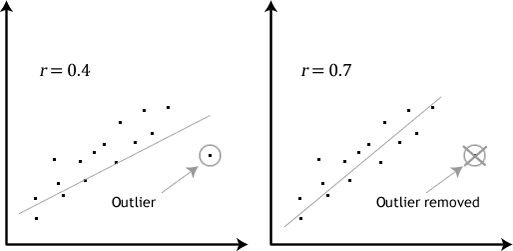
\includegraphics[width=0.7\linewidth]{images/pearson-outliers}
\caption{}
\label{fig:pearson-outliers}
\end{figure}


Pearson’s correlation coefficient, r, is sensitive to outliers, which can have a very large effect on the line of best fit and the Pearson correlation coefficient. Therefore, in some cases, including outliers in your analysis can lead to misleading results. 

Therefore, it is best if there are no outliers or they are kept to a minimum. Fortunately, when using SPSS Statistics to run Pearson’s correlation on your data, you can easily include procedures to screen for outliers. In our enhanced Pearson’s correlation guide, we: (a) show you how to detect outliers using a scatterplot, which is a simple process when using SPSS Statistics; and (b) discuss some of the options available to you in order to deal with outliers.

\begin{description}
	\item[Assumption 4:] Your variables should be approximately normally distributed. In order to assess the statistical significance of the Pearson correlation, you need to have bivariate normality, but this assumption is difficult to assess, so a simpler method is more commonly used. This simpler method involves determining the normality of each variable separately. To test for normality you can use the Shapiro-Wilk test of normality, which is easily tested for using SPSS Statistics. In addition to showing you how to do this in our enhanced Pearson’s correlation guide, we also explain what you can do if your data fails this assumption.
\end{description}

You can check assumptions 2, 3 and 4 using SPSS Statistics. Remember that if you do not test these assumptions correctly, the results you get when running a Pearson's correlation might not be valid. This is why we dedicate a number of sections of our enhanced Pearson's correlation guide to help you get this right. You can find out about our enhanced content as a whole here, or more specifically, learn how we help with testing assumptions here.

In the section, Test Procedure in SPSS Statistics, we illustrate the SPSS Statistics procedure to perform a Pearson’s correlation assuming that no assumptions have been violated. First, we set out the example we use to explain the Pearson’s correlation procedure in SPSS Statistics.

%=========================================================%
\subsection{Example}
A researcher wants to know whether a person's height is related to how well they perform in a long jump. The researcher recruited untrained individuals from the general population, measured their height and had them perform a long jump. The researcher then investigated whether there was an association between height and long jump performance by running a Pearson's correlation.

%=========================================================%
\subsection{Setup in SPSS Statistics}
In SPSS Statistics, we created two variables so that we could enter our data: \texttt{Height} (i.e., participants' height) and \texttt{Jump\_Dist} (i.e., distance jumped in a long jump). In our enhanced Pearson's correlation guide, we show you how to correctly enter data in SPSS Statistics to run a Pearson's correlation. You can learn about our enhanced data setup content here. Alternately, we have a generic, "quick start" guide to show you how to enter data into SPSS Statistics, available here.

%=========================================================%
\subsection*{Test Procedure in SPSS Statistics}
The six steps below show you how to analyse your data using Pearson’s correlation in SPSS Statistics when none of the four assumptions in the Assumptions section have been violated. At the end of these six steps, we show you how to interpret the results from this test. If you are looking for help to make sure your data meets assumptions 2, 3 and 4, which are required when using Pearson’s correlations and can be tested using SPSS Statistics, you can learn more about our enhanced guides here.

Click Analyze > Correlate > Bivariate... on the main menu, as shown below:

The SPSS Statistics Pearson Correlation Menu
\begin{figure}
\centering
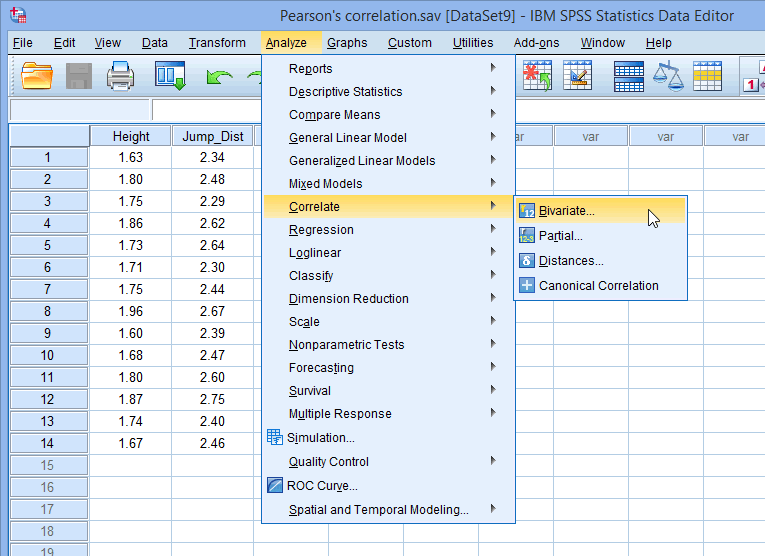
\includegraphics[width=0.7\linewidth]{images/pearsons-correlation-menu}
\caption{}
\label{fig:pearsons-correlation-menu}
\end{figure}

You will be presented with the Bivariate Correlations dialogue box:

The SPSS Statistics Bivariate Correlation Dialogue Box
\begin{figure}
\centering
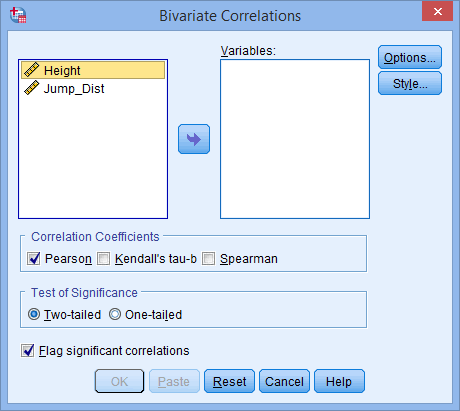
\includegraphics[width=0.7\linewidth]{images/pearsons-correlation-dialogue-box}
\caption{}
\label{fig:pearsons-correlation-dialogue-box}
\end{figure}

Transfer the variables \texttt{Height} and \texttt{Jump\_Dist} into the Variables: box by dragging-and-dropping them or by clicking on them and then clicking the SPSS Right Arrow Button button. You will end up with a screen similar to the one below:

The SPSS Statistics Bivariate Correlation Dialogue Box with Variables Transferred
\begin{figure}
	\centering
	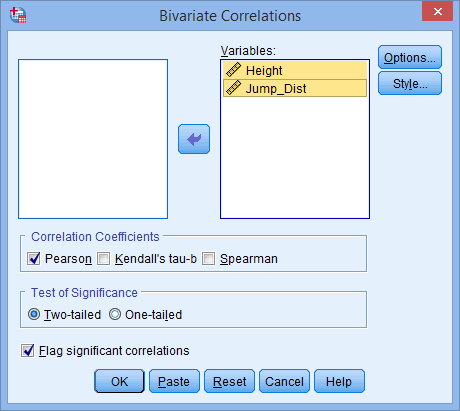
\includegraphics[width=0.7\linewidth]{images/pearsons-correlation-transferred}
	\caption{}
	\label{fig:pearsons-correlation-transferred}
\end{figure}

Note: If you study involves calculating more than one correlation and you want to carry out these correlations at the same time, we show you how to do this in our enhanced Pearson’s correlation guide. We also show you how to write up the results from multiple correlations.

Make sure that the Pearson checkbox is selected under the –Correlation Coefficients– area (although it is selected by default in SPSS Statistics).

Click the SPSS Options Button button and you will be presented with the Bivariate Correlations: Options dialogue box. If you wish to generate some descriptives, you can do it here by clicking on the relevant checkbox in the –Statistics– area.

The SPSS Statistics Bivariate Correlation Options Dialogue Box
Published with written permission from SPSS Statistics, IBM Corporation.
Click the  button. You will be returned to the Bivariate Correlations dialogue box.

Click the  button. This will generate the results of Pearson's correlation.

%=========================================================%
\subsection{Output for Pearson's correlation}
\begin{itemize}
	\item SPSS Statistics generates a single Correlations table that contains the results of the Pearson’s correlation procedure that you ran in the previous section.
	\item If your data passed assumption 2 (linear relationship), assumption 3 (no outliers) and assumption 4 (normality), which we explained earlier in the Assumptions section, you will only need to interpret this one table. 
	\item However, since you should have tested your data for these assumptions, you will also need to interpret the SPSS Statistics output that was produced when you tested for them (i.e., you will have to interpret: (a) the scatterplot you used to check for a linear relationship between your two variables; (b) the scatterplot that you used to assess whether there were any significant outliers; and (c) the output SPSS Statistics produced for your Shapiro-Wilk test of normality). 
	\item If you do not know how to do this, we show you in our enhanced Pearson’s correlation guide. Remember that if your data failed any of these assumptions, the output that you get from the Pearson’s correlation procedure (i.e., the table we discuss below) will no longer be correct.
	
\end{itemize}

However, in this "quick start" guide, we focus on the results from the Pearson’s correlation procedure only, assuming that your data met all the relevant assumptions. Therefore, when running the Pearson’s correlation procedure, you will be presented with the Correlations table in the IBM SPSS Statistics Output Viewer. The Pearson's correlation result is highlighted below:

\subsection{The Pearson Product-Moment Correlation}
\begin{figure}
\centering
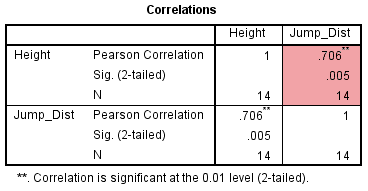
\includegraphics[width=0.7\linewidth]{images/pearsons-correlation-result-highlighted}
\caption{}
\label{fig:pearsons-correlation-result-highlighted}
\end{figure}

The results are presented in a matrix such that, as can be seen above, the correlations are replicated. Nevertheless, the table presents the Pearson correlation coefficient, its significance value and the sample size that the calculation is based on.

In this example, we can see that the Pearson correlation coefficient, r, is 0.706, and that it is statistically significant (p = 0.005). 

%=========================================================%
\subsection{Reporting the Output}
In our example above, you might report the results as follows:

General
A Pearson product-moment correlation was run to determine the relationship between height and distance jumped in a long jump. There was a strong, positive correlation between height and distance jumped, which was statistically significant (r = .706, n = 14, p = .005).

In our enhanced Pearson’s correlation guide, we also show you how to write up the results from your assumptions tests and Pearson’s correlation output if you need to report this in a dissertation, thesis, assignment or research report. We do this using the Harvard and APA styles. We also show you how to write up your results if you have performed multiple Pearson’s correlations. You can learn more about our enhanced content here.

%==========================================================%

\section{Spearman's Rank-Order Correlation using SPSS Statistics}

\subsection{Introduction}
\begin{itemize}
	\item The Spearman rank-order correlation coefficient (Spearman’s correlation, for short) is a nonparametric measure of the strength and direction of association that exists between two variables measured on at least an ordinal scale. 
	\item It is denoted by the symbol rs (or the Greek letter ρ, pronounced rho). The test is used for either ordinal variables or for continuous data that has failed the assumptions necessary for conducting the Pearson's product-moment correlation.
	\item  For example, you could use a Spearman’s correlation to understand whether there is an association between exam performance and time spent revising; whether there is an association between depression and length of unemployment; and so forth. If you would like some more background on this test, you can find it here. Possible alternative tests to Spearman's correlation are Kendall's tau-b or Goodman and Kruskal's gamma.
\end{itemize}





\subsection{Assumptions}
When you choose to analyse your data using Spearman’s correlation, part of the process involves checking to make sure that the data you want to analyse can actually be analysed using a Spearman’s correlation. You need to do this because it is only appropriate to use a Spearman’s correlation if your data "passes" two assumptions that are required for Spearman’s correlation to give you a valid result. In practice, checking for these two assumptions just adds a little bit more time to your analysis, requiring you to click of few more buttons in SPSS Statistics when performing your analysis, as well as think a little bit more about your data, but it is not a difficult task. These two assumptions are:
\begin{description}
	\item[Assumption 1:] Your two variables should be measured on an ordinal, interval or ratio scale. Examples of ordinal variables include Likert scales (e.g., a 7-point scale from "strongly agree" through to "strongly disagree"), amongst other ways of ranking categories (e.g., a 3-pont scale explaining how much a customer liked a product, ranging from "Not very much", to "It is OK", to "Yes, a lot"). Examples of interval/ratio variables include revision time (measured in hours), intelligence (measured using IQ score), exam performance (measured from 0 to 100), weight (measured in kg), and so forth. You can learn more about ordinal, interval and ratio variables in our article: Types of Variable.
	\item[Assumption 2:] There is a monotonic relationship between the two variables. A monotonic relationship exists when either the variables increase in value together, or as one variable value increases, the other variable value decreases. Whilst there are a number of ways to check whether a monotonic relationship exists between your two variables, we suggest creating a scatterplot using SPSS Statistics, where you can plot one variable against the other, and then visually inspect the scatterplot to check for monotonicity. Your scatterplot may look something like one of the following:
\end{description}


\subsection{Examples of Relationships}
\begin{itemize}
	\item The relationship displayed in your scatterplot should be monotonic. In our enhanced guides, we show you how to: (a) create a scatterplot to check for a monotonic relationship when carrying out Spearman’s correlation using SPSS Statistics; (b) interpret different scatterplot results; and (c) consider possible solutions if your data fails this assumption. Just remember that if you do not test these assumptions correctly, the results you get when running a Spearman's correlation might not be valid. This is why we dedicate a number of sections of our enhanced Spearman's correlation guide to help you get this right. You can find out about our enhanced content as a whole here, or more specifically, learn how we help with testing assumptions here. 
	
\item Note: Spearman's correlation determines the degree to which a relationship is monotonic. Put another way, it determines whether there is a monotonic component of association between two continuous or ordinal variables. As such, monotonicity is not actually an assumption of Spearman's correlation. However, you would not normally want to pursue a Spearman's correlation to determine the strength and direction of a monotonic relationship when you already know the relationship between your two variables is not monotonic. 
\item Instead, the relationship between your two variables might be better described by another statistical measure of association. For this reason, it is not uncommon to view the relationship between your two variables in a scatterplot to see if running a Spearman's correlation is the best choice as a measure of association or whether another measure would be better.
\item In terms of assumption 2 above, you can check this using SPSS Statistics. If your two variables do not appear to have a monotonic relationship, you might consider using a different statistical test, which we show you how to do in our Statistical Test Selector (N.B., this is part of our enhanced content).
	
\item It is also worth noting that a Spearman’s correlation can be used when your two variables are not normally distributed. It is also not very sensitive to outliers, which are observations within your data that do not follow the usual pattern. Since Spearman’s correlation is not very sensitive to outliers, this means that you can still obtain a valid result from using this test when you have outliers in your data.
	
\end{itemize}

In the section, Test Procedure in SPSS Statistics, we illustrate the SPSS Statistics procedure to perform a Spearman’s correlation assuming that no assumptions have been violated. First, we set out the example we use to explain the Spearman’s correlation procedure in SPSS Statistics.

%========================================================%
\subsection{Example}
A teacher is interested in whether those who do better at English also do better in maths. To test whether this is the case, the teacher records the scores of her 10 students in their end-of-year examinations for both English and maths. Therefore, one variable records the English scores and the second variable records the maths scores for the 10 pupils.


%========================================================%
\subsection{Setup in SPSS Statistics}
In SPSS Statistics, we created two variables so that we could enter our data: E\texttt{nglish\_Mark} (i.e., English scores) and \texttt{Maths\_Mark} (i.e., maths scores). In our enhanced Spearman's correlation guide, we show you how to correctly enter data in SPSS Statistics to run a Spearman's correlation. You can learn about our enhanced data setup content here. Alternately, we have a generic, "quick start" guide to show you how to enter data into SPSS Statistics, available here.


%========================================================%
\subsection{Test Procedure in SPSS Statistics}
The four steps below show you how to analyse your data using Spearman’s correlation in SPSS Statistics when neither of the two assumptions in the previous section, Assumptions, have been violated. At the end of these four steps, we show you how to interpret the results from this test. If you are looking for help to assess whether the relationship between your two variables is monotonic, we show you how to do this in our enhanced guide. You can learn more about our enhanced guides here.

Click Analyze > Correlate > Bivariate... on the main menu as shown below:
\begin{figure}
\centering
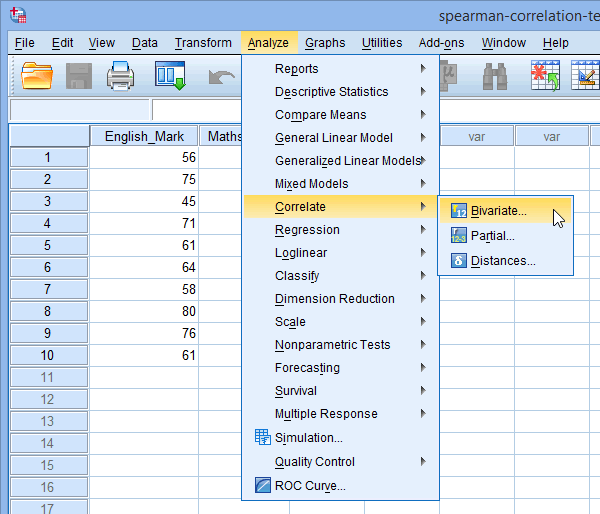
\includegraphics[width=0.7\linewidth]{images/spearmans-rank-order-correlation-1}
\caption{}
\label{fig:spearmans-rank-order-correlation-1}
\end{figure}

Spearman's Rank Order Correlation
%Published with written permission from SPSS Statistics, IBM Corporation.
You will be presented with the following Bivariate Correlations dialogue box:
\begin{figure}
\centering
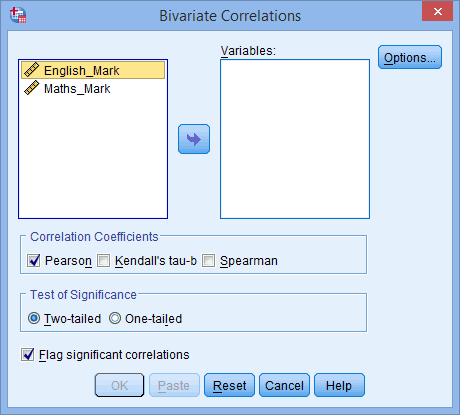
\includegraphics[width=0.7\linewidth]{images/spearmans-rank-order-correlation-2}
\caption{}
\label{fig:spearmans-rank-order-correlation-2}
\end{figure}

Spearman's Rank Order Correlation
Published with written permission from SPSS Statistics, IBM Corporation.
Transfer the variables \texttt{English\_Mark} and \texttt{Maths\_Mark} into the Variables: box by dragging-and-dropping the variables or by clicking each variable and then clicking the SPSS Right Arrow Button button. You will end up with a screen similar to the one below:
\begin{figure}
	\centering
	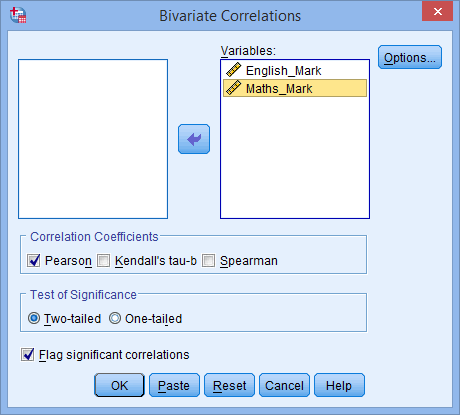
\includegraphics[width=0.7\linewidth]{images/spearmans-rank-order-correlation-3}
	\caption{}
	\label{fig:spearmans-rank-order-correlation-3}
\end{figure}
Spearman's Rank Order Correlation
Published with written permission from SPSS Statistics, IBM Corporation.
Make sure that you uncheck the Pearson checkbox (it is selected by default in SPSS Statistics) and select the Spearman checkbox in the –Correlation Coefficients– area. You will end up with a screen similar to below:

Spearman's Rank Order Correlation
Published with written permission from SPSS Statistics, IBM Corporation.
Click the  button. This will generate the results.

%=========================================================%
\subsection{Output}
SPSS Statistics generates a single table following the Spearman’s correlation procedure that you ran in the previous section. If your data passed assumption 2 (i.e., there is a monotonic relationship between your two variables), you will only need to interpret this one table. However, since you should have tested your data for monotonicity, you will also need to interpret the SPSS Statistics output that was produced when you tested for it (i.e., your scatterplot results). If you do not know how to do this, we show you in our enhanced Spearman’s correlation guide. 

If you have tested your data for these assumptions, we provide a complete explanation of the output you will have to interpret in our enhanced Spearman’s guide. Remember that if your data failed this assumption, the output that you get from the Spearman’s correlation procedure (i.e., the table we discuss below), might be misleading.

However, in this "quick start" guide, we focus on the results from the Spearman’s correlation procedure only. Therefore, after running the Spearman’s correlation procedure, you will be presented with the Correlations table, as shown below:

\subsection{Spearman's Rank Order Correlation}
Published with written permission from SPSS Statistics, IBM Corporation.
The results are presented in a matrix such that, as can be seen above, the correlations are replicated. Nevertheless, the table presents Spearman's correlation, its significance value and the sample size that the calculation was based on. In this example, we can see that Spearman's correlation coefficient, rs, is 0.669, and that this is statistically significant (p = .035).

%=======================================================%
Reporting the Output
In our example, you might present the results as follows:

General
A Spearman's rank-order correlation was run to determine the relationship between 10 students' English and maths exam marks. There was a strong, positive correlation between English and maths marks, which was statistically significant (rs(8) = .669, p = .035).

In our enhanced Spearman’s correlation guide, we also show you how to write up the results from your assumptions test and Spearman’s correlation output if you need to report this in a dissertation, thesis, assignment or research report. We do this using the Harvard and APA styles. You can learn more about our enhanced content here.




\section{Kendall's Tau-b using SPSS Statistics}

\subsection{Introduction}
Kendall's tau-b (τb) correlation coefficient (Kendall's tau-b, for short) is a nonparametric measure of the strength and direction of association that exists between two variables measured on at least an ordinal scale. It is considered a nonparametric alternative to the Pearson’s product-moment correlation when your data has failed one or more of the assumptions of this test. It is also considered an alternative to the nonparametric Spearman rank-order correlation coefficient (especially when you have a small sample size with many tied ranks). If you consider one of your variables as an independent variable and the other as a dependent variable, you might consider running a Somers' d test instead.

For example, you could use Kendall's tau-b to understand whether there is an association between exam grade and time spent revising (i.e., where there were six possible exam grades – A, B, C, D, E and F – and revision time was split into five categories: less than 5 hours, 5-9 hours, 10-14 hours, 15-19 hours, and 20 hours or more). Alternately, you could use Kendall's tau-b to understand whether there is an association between customer satisfaction and delivery time (i.e., where delivery time had four categories – next day, 2 working days, 3-5 working days, and more than 5 working days – and customer satisfaction was measured in terms of the level of agreement customers had with the following statement, "I am satisfied with the time it took for my parcel to be delivered", where the level of agreement had five categories: strongly agree, agree, neither agree nor disagree, disagree and strongly disagree).

This "quick start" guide shows you how to carry out Kendall's tau-b using SPSS Statistics. We show you the main procedure for doing this here. However, first we introduce you to the assumptions that you must consider when carrying out Kendall's tau-b.

\subsection{Assumptions}
When you choose to analyse your data using Kendall's tau-b, part of the process involves checking to make sure that the data you want to analyse can actually be analysed using Kendall's tau-b. You need to do this because it is only appropriate to use Kendall's tau-b if your data "passes" the assumptions that are required for Kendall's tau-b to give you a valid result. In practice, checking for these assumptions just adds a little bit more time to your analysis, requiring you to click of few more buttons in SPSS Statistics when performing your analysis, as well as think a little bit more about your data, but it is not a difficult task. These two assumptions are:

Assumption 1: Your two variables should be measured on an ordinal or continuous scale. Examples of ordinal variables include Likert scales (e.g., a 7-point scale from strongly agree through to strongly disagree), amongst other ways of ranking categories (e.g., a 5-point scale explaining how much a customer liked a product, ranging from "Not very much" to "Yes, a lot"). Examples of continuous variables (i.e., interval or ratio variables) include revision time (measured in hours), intelligence (measured using IQ score), exam performance (measured from 0 to 100), weight (measured in kg), and so forth. You can learn more about ordinal and continuous variables in our article: Types of Variable.
Assumption 2: Kendall's tau-b determines whether there is a monotonic relationship between your two variables. As such, it is desirable if your data would appear to follow a monotonic relationship, so that formally testing for such an association makes sense, but it is not a strict assumption or one that you are often able to assess.
In the section, Test Procedure in SPSS Statistics, we illustrate the SPSS Statistics procedure to perform Kendall's tau-b assuming that no assumptions have been violated. First, we set out the example we use to explain the Kendall's tau-b procedure in SPSS Statistics.

%========================================================%
\subsection{Example \& Data Setup in SPSS Statistics}
Taxes have the ability to elicit strong responses in many people, with some thinking they are too high, whilst others think they should be higher. A researcher conducted a simple study where they presented participants with the statement: "Tax is too high in this country", and asked them how much they agreed with this statement. They had four options how to respond: "Strongly Disagree", "Disagree", "Agree" or "Strongly Agree". These ordered responses were the categories of the dependent variable, \texttt{tax\_too\_high}. The researcher also asked participants to state whether they had a "low", "middle" or "high" income, where each of these categories had specified income ranges (e.g., a low income was any income under £18,000 per annum). The income level of participants was recorded in the variable, income.

Therefore, in the Variable View of SPSS Statistics two ordinal variables were created so that the data collected could be entered: income and \texttt{tax\_too\_high}. Next, the data from 24 participants was entered into the Data View of SPSS Statistics.


\subsection{Test Procedure in SPSS Statistics}
The four steps below show you how to analyse your data using Kendall's tau-b in SPSS Statistics when neither of the two assumptions in the previous section, Assumptions, have been violated. At the end of these four steps, we show you how to interpret the results from this test.

Click Analyze > Correlate > Bivariate... on the top menu, as shown below:

\subsection{Kendall's tau-b}
Published with written permission from SPSS Statistics, IBM Corporation.
You will be presented with the Bivariate Correlations dialogue box, as shown below:

Kendall's tau-b
\begin{figure}
\centering
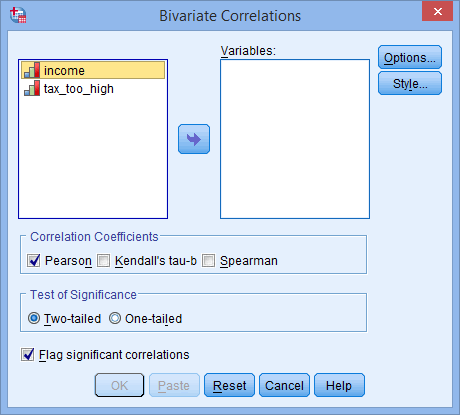
\includegraphics[width=0.7\linewidth]{images/options-kendalls-tau-b}
\caption{}
\label{fig:options-kendalls-tau-b}
\end{figure}

Transfer the variables income and \texttt{tax\_too\_high} into the Variables: box by dragging-and-dropping or by clicking the SPSS Right Arrow Button button. You will end up with a screen similar to the one below:
\begin{figure}
\centering
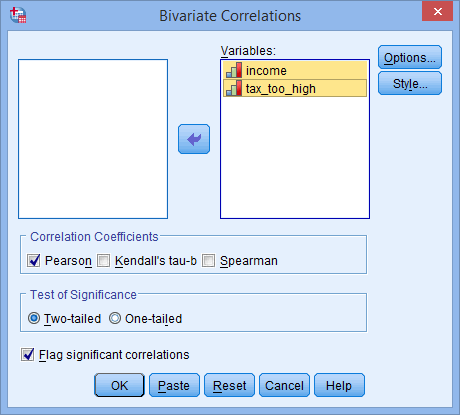
\includegraphics[width=0.7\linewidth]{images/options-example-kendalls-tau-b}
\caption{}
\label{fig:options-example-kendalls-tau-b}
\end{figure}

Kendall's tau-b
%%Published with written permission from SPSS Statistics, IBM Corporation.
Make sure that you uncheck the Pearson tick box (it is selected by default in SPSS Statistics) and check the Kendall's tau-b tick box in the –Correlation Coefficients– area, as shown below:
\begin{figure}
\centering
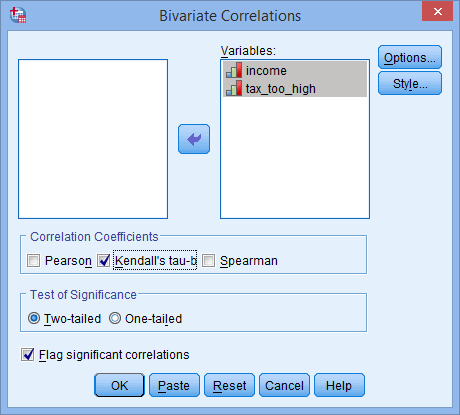
\includegraphics[width=0.7\linewidth]{images/options-example-2-kendalls-tau-b}
\caption{}
\label{fig:options-example-2-kendalls-tau-b}
\end{figure}

Kendall's tau-b
Published with written permission from SPSS Statistics, IBM Corporation.
Click the  button.

%=======================================================%
\subsection{Interpreting the Results for Kendall's Tau-b}
SPSS Statistics generates one main table for the Kendall's tau-b procedure that you ran in the previous section. If your data passed assumption 2 (i.e., there is a monotonic relationship between your two variables), which we explained earlier in the Assumptions section, you will only need to interpret this one table. However, since you should have tested your data for this assumption, you will also need to interpret the SPSS Statistics output that was produced when you tested for it (i.e., your scatterplot results). Remember that if your data failed this assumption, the output that you get from the Kendall's tau-b procedure (i.e., the table we discuss below) will no longer be correct.

In this "quick start" guide we focus on the results from the Kendall's tau-b procedure only, assuming that your data met this assumption. Therefore, when running the Kendall's tau-b procedure, you will be presented with the table below, entitled Correlations:

Kendall's tau-b
Published with written permission from SPSS Statistics, IBM Corporation.
The results are presented in a matrix such that, as can be seen, the correlations are replicated. Nevertheless, the table presents Kendall's tau-b correlation, its significance value and the sample size that the calculation was based on. In this example, we can see that Kendall's tau-b correlation coefficient, τb, is 0.535, and that this is statistically significant (p = 0.003).

%=========================================================%
Reporting the Results for Kendall's Tau-b
In our example, you might present the results as follows:

General
A Kendall's tau-b correlation was run to determine the relationship between income level and views towards income taxes amongst 24 participants. There was a strong, positive correlation between income level and the view that taxes were too high, which was statistically significant (τb = .535, p = .003).



\end{document}